\chapter{Results}
\label{chap:results}
The datasheet of our \ce{NdFeB} particles specifies that their residual magnetic field is \qtyrange{730}{760}{\milli\tesla}. Full saturation (\qty{>95}{\percent}) is achieved when a \qty{2}{\tesla} field is applied\cite{magnequench}. Our method of magnetizing the particle was limited to a \qty{1.4}{\tesla} field. As such, it is likely that we did not achieve the full saturation of the particle and that the residual magnetic field is lower than specified. Assuming a roughly linear relation between the two values, we estimate the residual magnetic field of our particles to be \qtyrange{510}{530}{\milli\tesla}. The density of the particles is given as \qty{7430}{\kilo\gram\per\cubic\meter}\cite{magnequench}.

These values, together with the simulation of the magnetic field distribution in the trap, allow us to estimate the required driving frequency and the resulting eigenfrequency. \autoref{fig:magnetic-field-curvature} shows the $z$-component of the ac magnetic field ($\vec{B_1}$) for a range of $\xi$ values as well as the curvature. It is important to note that the \xmode and \ymode have a negative curvature, whilst the \zmode has a positive curvature. This means that $x$ and $y$ are not stable. Half a period later however this will have changed, and the particle will be stable in the $x$- and $y$-direction instead of the $z$-direction. This is what leads to the ponderomotive effect. The curves for $y$ are not symmetric because the slit is in the direction of the \ymode.

Using \autoref{eq:eigenfrequencies} and \autoref{eq:frequency-constraint} we can then estimate the required driving frequency and the resulting eigenfrequencies. These results are shown in \autoref{fig:eigen-frequency-xi-dependence}.

\begin{figure}
    \centering
    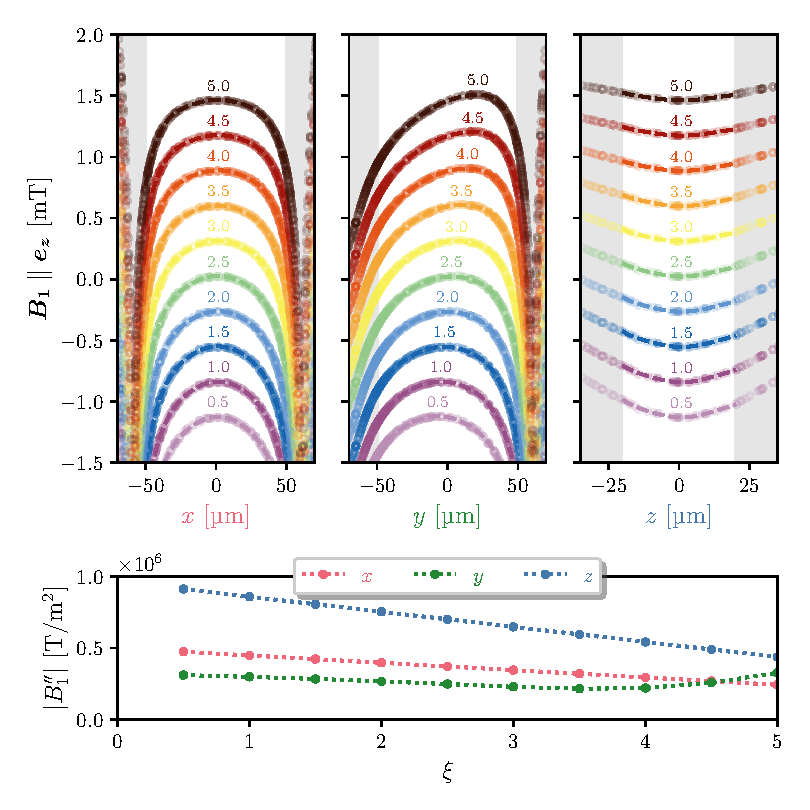
\includegraphics{figures/data/magnetic_field_curvature.pdf}
    \caption{The \textbf{top} figures from left to right show $z$-component of the magnetic field evaluated along a line parallel to the $x$-, $y$- and $z$-axis respectively through the origin. The gray zones indicate the boundaries of the trap. The \textbf{bottom left} figure shows the curvature of the magnetic field for these calculations evaluated in the extrema. The simulations were performed for $i_1=\qty{0.5}{\ampere}$ and $\xi$ between \numrange{0.5}{5}. The curves have been labelled with the corresponding value for $\xi$. In addition to this the offset in $y$ due to the trap asymmetry is shown in the \textbf{bottom right} figure.}
    \label{fig:magnetic-field-curvature}
\end{figure}

\begin{figure}
    \centering
    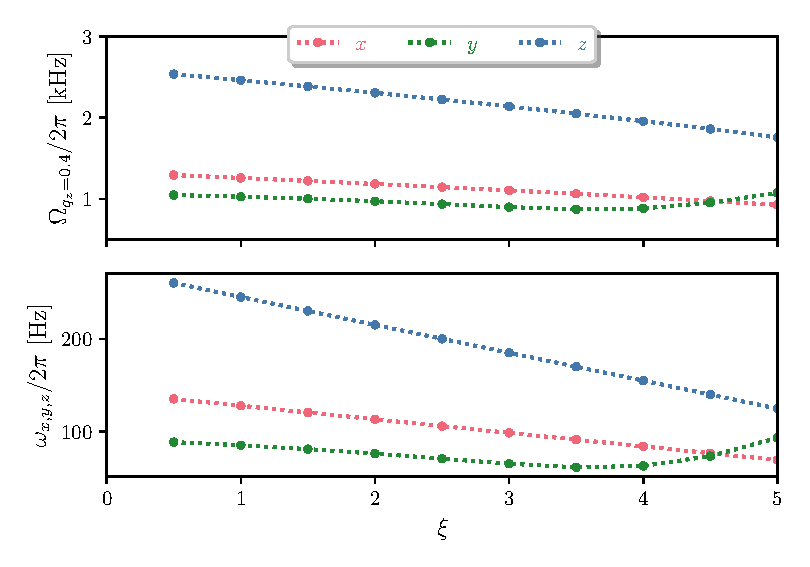
\includegraphics{figures/data/eigen_frequency_xi_dependence.pdf}
    \caption{Simulation results of the dependence of the eigenfrequency on $\xi$. These results are based on the data presented in \autoref{fig:magnetic-field-curvature}. The \textbf{top} figure shows the minimal trapping frequency such that $q_z \leq 0.4$. In the \textbf{middle} the corresponding eigenfrequencies of the modes are shown for $\Omega / 2\pi = \qty{2.5}{\kilo\hertz}$. The \textbf{bottom} figure shows the deviation from the centre of the \ymode. The dashed lines are a linear interpolation of the data and only serve as a guide to the eyes.}
    \label{fig:eigen-frequency-xi-dependence}
\end{figure}

\section{Measurements at atmospheric pressure}
\label{sec:measurements-at-atmospheric-pressure}
At atmospheric pressure we determined the dependence of $\omega_{x,y}$ on $\Omega$ and $i_1$. In these measurements the ratio $\xi=2$ was kept constant. The spectra are obtained using the laser readout scheme. Due to the low Q-factor at atmospheric pressure, it is not possible to tell the $x$- and $y$-modes apart. The results are shown in \autoref{fig:xy-mode-dependence-driving-frequency-1bar} and \autoref{fig:xy-mode-dependence-inner-current-1bar}. The $z$-mode is not visible in these measurements. The observed Q-factors are very low, hence the very broad peaks. This is also the reason we cannot clearly discern the \xmode from the \ymode. In addition to this the dependence of the librational mode on $B_0$ is shown in \autoref{fig:librational-mode-dependence-magnetic-field-1bar}. We note three curves with a apparently linear dependence on $B_0$. The two additional curves are modulations of the resonance peak with the trapping frequency. A fourth curve can be seen in the bottom right. Its origin is unclear. A fit has not been made due to the sparsity of the data. $\omega_\alpha$ has not been observed.

\begin{SCfigure}[][h]
    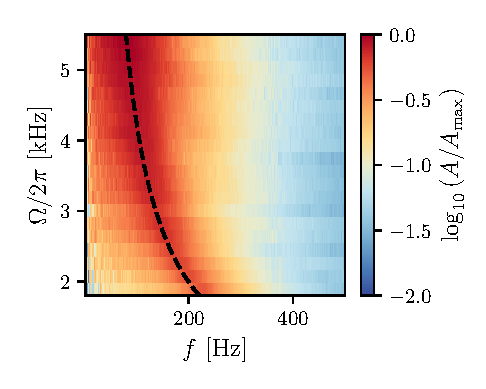
\includegraphics{figures/data/xy_mode_dependence_on_driving_frequency.pdf}
    \caption{Dependence of $\omega_{x,y}$ on $\Omega$ at atmospheric pressure. The dashed line is a fit as expected from the theory of $\omega_{x,y} \propto 1/\Omega$. We used $i_1 = \qty{200}{\milli\ampere}$ and $\xi = 2$.}
    \label{fig:xy-mode-dependence-driving-frequency-1bar}
\end{SCfigure}
\begin{SCfigure}[][h]
    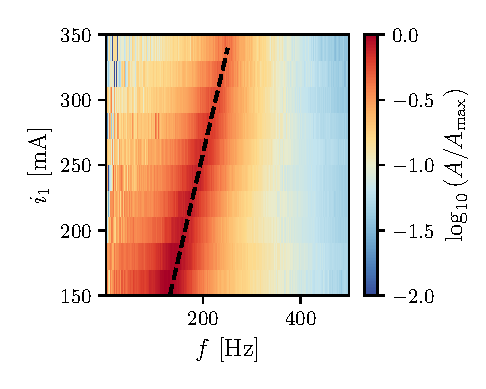
\includegraphics{figures/data/xy_mode_dependence_on_inner_current.pdf}
    \caption{Dependence of $\omega_{x,y}$ on $i_1$ at atmospheric pressure. The dashed line is a fit as expected from the theory of $\omega_{x,y} \propto i_1$. We used $\Omega/2\pi = \qty{2.5}{\kilo\hertz}$ and $\xi = 2$.}
    \label{fig:xy-mode-dependence-inner-current-1bar}
\end{SCfigure}
\begin{SCfigure}[][h]
    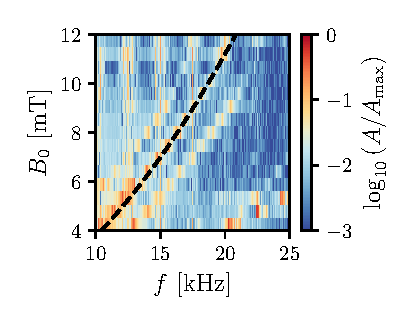
\includegraphics{figures/data/librational_mode_dependence_on_B0.pdf}
    \caption{Dependence of $\omega_{\gamma,\beta}$ on $B_0$ at atmospheric pressure. The dashed line is a manual fit as expected from the theory of $\omega_{\gamma,\beta} \propto \sqrt{B_0}$. The magnitude of the field has been determined based on the current through the Helmholtz coil and converted using the calibration data in the supplementary data of \textcite{janse_characterization_2024}.}
    \label{fig:librational-mode-dependence-magnetic-field-1bar}
\end{SCfigure}

\section{Measurements at low pressure}
\label{sec:measurements-at-low-pressure}
At \qty{1}{\milli\bar} the readout was performed using the Thorcam and analysed using our custom object tracking algorithm. The reason to no longer use laser readout is due to the heating of the particle. By equating the power of the laser to Stefan-Boltzmann law we find that, in equilibrium assuming no heat dissipation through air, the temperature of the particle could reach \qty{2500}{\kelvin}. Even if only a fraction of the laser power would reach the particle this would be enough to reach its Curie temperature of \qty{320}{\celsius}\cite{magnequench}. Lower laser powers leads to an insufficient signal-to-noise ratio. We will return to this in the discussion. For a more thorough analysis of heating refer to \cite{millen}.

\begin{SCfigure}[][h]
    \centering
    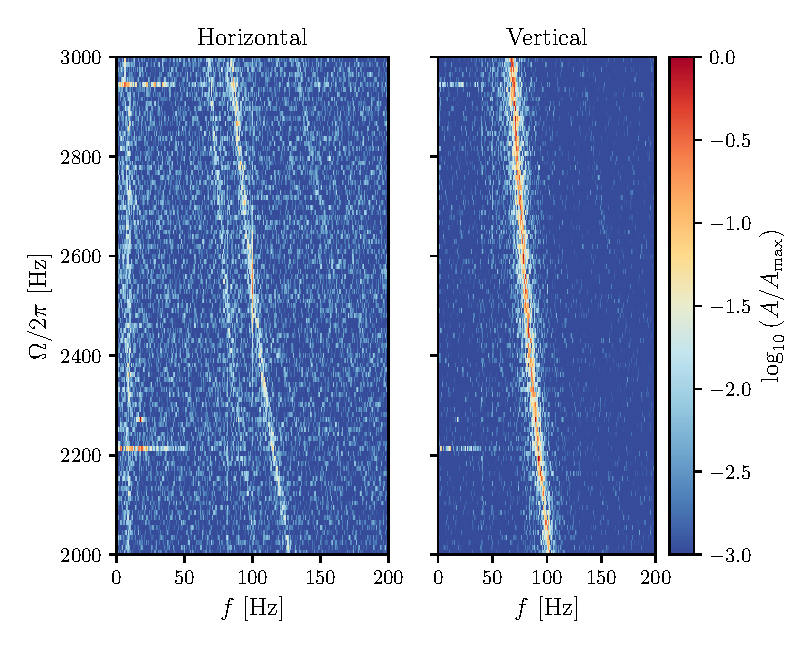
\includegraphics{figures/data/xyz_mode_dependence_on_driving_frequency_spectrum.pdf}
    \caption{The dependence of $\omega_{x,y,z}$ on $\Omega$ at \qty{1}{\milli\bar}. Shown are two directions (horizontal and vertical), they live in the $xy$-plane but do not directly match to the \xmode or \ymode, a small rotation angle needs to be taken into account.}
    \label{fig:xyz-mode-dependence-1mbar}
\end{SCfigure}

\autoref{fig:xyz-mode-dependence-1mbar} shows the dependence of $\omega_{x,y,z}$ at \qty{1}{\milli\bar}. We note that compared to the measurements at atmospheric pressures that the width of the peak is substantially smaller. Whilst this measurement shows a clear dependence of $\omega_{x,y,z}$ on $\Omega$, it is very difficult to see the \zmode. These measurements were obtained by continuously sweeping the driving frequency. Instead, we can do a `lock-in like' measurement as described in \autoref{chap:method}. An example of such a measurement is shown in \autoref{fig:xyz-mode-spectrum-1mbar}.

\begin{SCfigure}[][h]
    \centering
    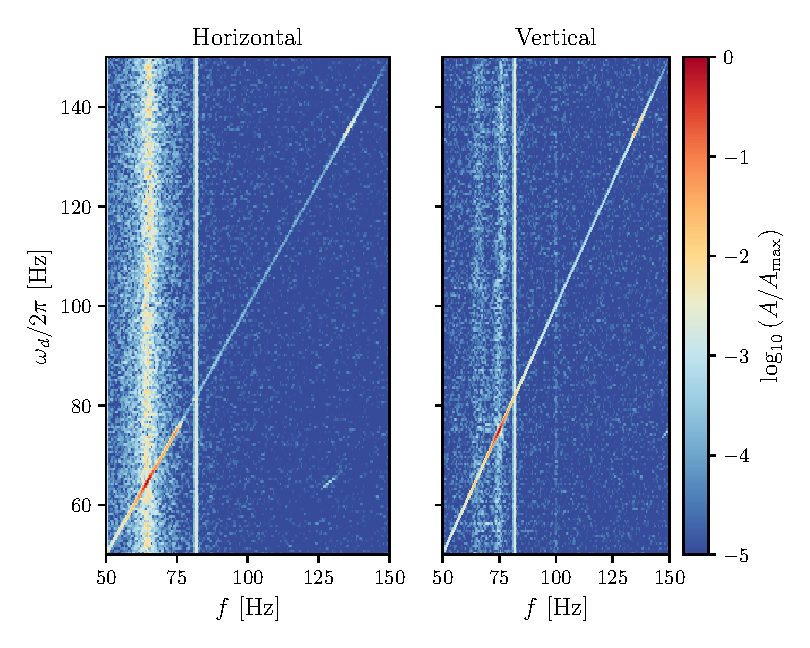
\includegraphics{figures/data/xyz_mode_spectrum.pdf}
    \caption{A PSD with a visible \xmode, \ymode and \zmode. The diagonal line is caused by the changing driving frequency. By looking at the magnitude along the diagonal line the eigenfrequencies and Q-factors can be determined after a Lorentzian fit.}
    \label{fig:xyz-mode-spectrum-1mbar}
\end{SCfigure}

By performing this `lock-in like' measurement at multiple driving frequencies we can determine clear relations between $\omega_{x,y,z}$, the damping and the driving frequency. We do so by fitting a Lorentzian for each peak in the spectrum. The results are shown in \autoref{fig:xyz-mode-dependence-on-trapping-frequency-1mbar}.

% The fits are given by:
% \begin{align*}
%     \omega_x &\propto \frac{\qty{ 11.394193305319426 \pm 0.6168138640026458 }{\square\kilo\hertz}}{\Omega} \\ % + (\qty{ -130.8583313665632 \pm 35.52389434927459 }{\hertz}) \\
%     \omega_y &\propto \frac{\qty{ 8.61031330605224 \pm 0.3506111962572132 }{\square\kilo\hertz}}{\Omega} \\ % + (\qty{ -47.01583771770941 \pm 21.39358314176167 }{\hertz}) \\
%     \omega_z &\propto \frac{\qty{ 19.211603271753344 \pm 0.9219280210953733 }{\square\kilo\hertz}}{\Omega} % + (\qty{ -142.4727024226977 \pm 53.88080820095942 }{\hertz})
% \end{align*}

\begin{figure}
    \centering
    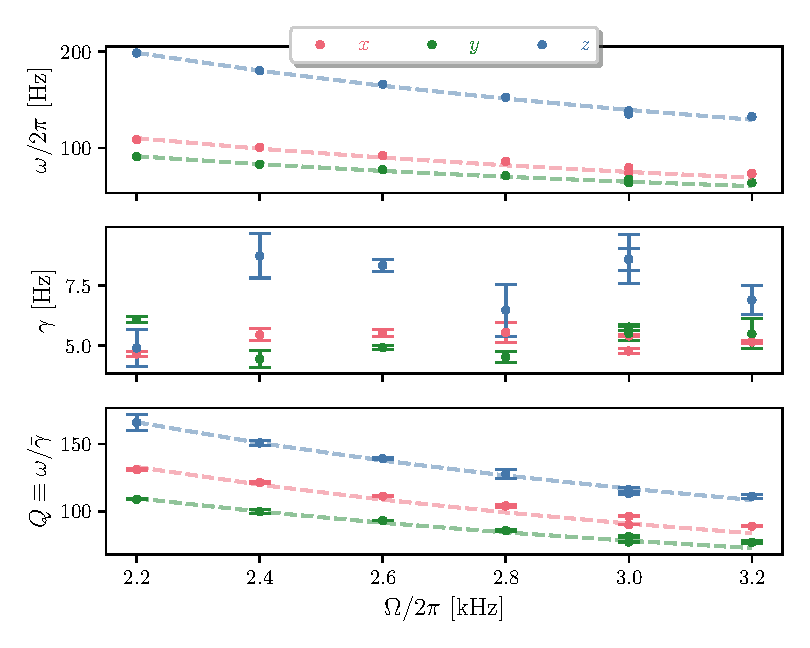
\includegraphics{figures/data/xyz_mode_dependence_on_driving_frequency.pdf}
    \caption{The dependence of $\omega_{x,y,z}$ and $\gamma_{x,y,z}$ on $\Omega$ at \qty{1}{\milli\bar}. The $\gamma$ in this case is the width of the Lorentzian fitted on the PSD. The dashed lines are a fit. The error bars are left out in the first figure because they are too small to be visible. The errorbars in the bottom figure are mostly dependent on the standard deviation on $\gamma$. The \zmode at $\Omega/2\pi = \qty{3}{\kilo\hertz}$ was determined in two separate measurements.}
    \label{fig:xyz-mode-dependence-on-trapping-frequency-1mbar}
\end{figure}

Visually it appears that $\gamma$ is constant as a function of $\Omega$. The question is whether $\gamma_z$ differs significantly from $\gamma_{x,y}$. To test this we perform a $T$-test on the mean values, the results can be found in \autoref{tab:gamma-t-test}. The T-test suggests that $\gamma_x = \gamma_y$ and $\gamma_z \gg \gamma_{x,y}$ at \qty{1}{\milli\bar}.

\begin{SCtable}[1]
    \centering
    \begin{tabular}{cc}
        \toprule
        $H_0$ & $p$ \\
        \midrule
        $\gamma_x = \gamma_y$ & \textcolor{x_axis_color}{$0.897 \gg 0.05$} \\
        $\gamma_y = \gamma_z$ & \textcolor{y_axis_color}{$0.005 \ll 0.05$} \\
        $\gamma_x = \gamma_z$ & \textcolor{y_axis_color}{$0.005 \ll 0.05$} \\
        \bottomrule
    \end{tabular}
    \caption{The results of the $T$-test on the mean values of $\gamma_{x,y,z}$ from the data in \autoref{fig:xyz-mode-dependence-on-trapping-frequency-1mbar}.}
    \label{tab:gamma-t-test}
\end{SCtable}

\section{Q-factor dependence on pressure}
\label{sec:q-factor-dependence-on-pressure}
Using an external coil we are able to excite the \xmode  and \ymode separately. Ringdown measurements are performed to determine the pressure dependence on the Q-factor. The Q-factor in this case is defined as $Q = \omega_{x,y,z} \tau / 2$ where $\tau$ is the decay time of the oscillation ($\sim \exp\left(t / \tau\right)$). We qualitatively observed a strong dependence of the Q-factor on the driving amplitude. When the driving amplitude is too high we observe non-linear time dependent behaviour. The results in \autoref{fig:q-factor-pressure-dependence} are obtained with a sufficiently low driving amplitude.

\begin{figure}[h]
    \centering
    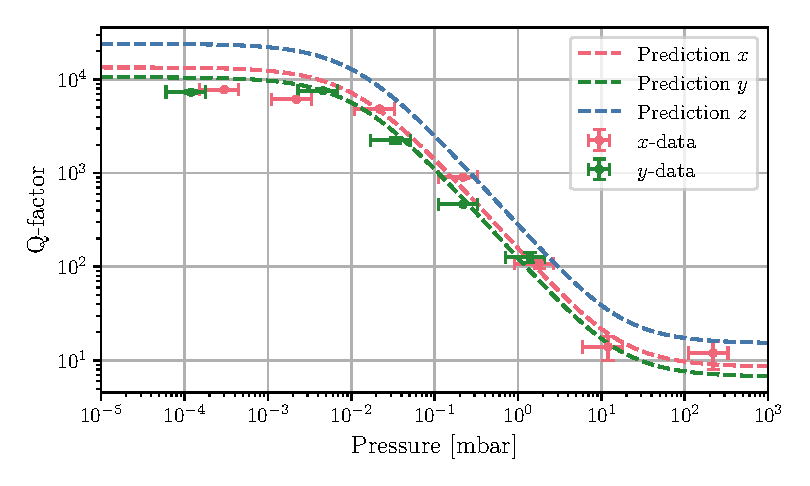
\includegraphics{figures/data/q_factor_pressure_dependence.pdf}
    \caption{The pressure dependence of the Q-factor for the $x$-, $y$- and $z$-mode. The dashed lines are a prediction based on the theory from \autoref{sec:damping}. The experimental Q-factors are determined using the ringdown method. The \zmode only been observed at \qty{1}{\milli\bar} and extrapolated from the data in \autoref{fig:xyz-mode-dependence-on-trapping-frequency-1mbar}. The driving frequency is $\Omega/2\pi = \qty{1.8}{\kilo\hertz}$.}
    \label{fig:q-factor-pressure-dependence}
\end{figure}

An attempt was made to model the damping at low pressures. This was done in COMSOL where we used the estimated maximum velocity of the particle as a Lorentz factor in the magnetic field. We considered two cases: the particle induced a current in the tracks and the particle induced a current in a \ce{Ga} layer of \qty{1}{\micro\meter} thick around the trap. The reason to model the \ce{Ga} layer is due to contamination during FIB milling. The results are shown in \autoref{tab:dissipation}. The dissipation of the \zmode is not included in this table because it has not been measured. Eddy current in the particle itself have not been taken into account.

\begin{table}
    \centering
    \begin{tabularx}{\textwidth}{Xccc}
        \toprule
        Source & \multicolumn{3}{c}{Dissipation (\unit{\atto\watt})} \\
        \cmidrule(r){2-4}
        & \xmode & \ymode & \zmode \\
        \midrule
        Ringdown measurements & \num{21.55 \pm 0.8} & \num{20.7 \pm 2.1} & --- \\
        \midrule
        Track dissipation sim. & \num{1.3878E-3} & \num{5.8018E-4} & \num{3.6026E-6} \\
        \ce{Ga} layer dissipation sim. & \num{0.595} & \num{0.393} & \num{0.272} \\
        % Thin wire model & \num{1.02} & \num{0.631} & \num{3.26} \\
        % Induction dissipation sim. & ??? & ??? & ??? \\
        \bottomrule
    \end{tabularx}
    \caption{The measured dissipation at low pressures ($<\qty{1E-3}{\milli\bar}$) for the \xmode and \ymode (data in \autoref{fig:q-factor-pressure-dependence}) compared to the simulated dissipation through induction and eddy currents in either the tracks and a thin \ce{Ga} layer.}
    \label{tab:dissipation}
\end{table}
